\chapter{Analysis}
After utilizing the AUSAlib tools, the data is ready to be analyzed. Even though the theory dictates that a decay will consist of two \al-particles and one \be-particles, it is not realistic to just assume that each detected event will consist only of this configuration of particles. \\
Therefore we need some cut on what events we will allow through to the analysis. Specifically we are going to impose 3 cuts on the data, a angular cut, a momentum cut and a multiplicity cut.

\section{Identifying the particles}
When a particle hits a given detector, we have no real knowledge of what particle it is. 
Therefore we need to do an analysis where we identify what particle we have.

This is done in \textcolor{red}{XX} steps
\subsection{Finding a hit}
The first step ind identifying a hit, is to actually get a hit, and gather the different properties of the specific hit. 

\subsection{Identifying a hit}
After a hit has been has been detected, and all the relevant information has been extracted from the hit, we can start to analyze what type of particle has hit the detector. 

A important distinction between an \al-particle and a \be-particle is the different interactions with a detector. An \al-particle will be completely stopped by a standard \SI{60}{\mu m} detector, while a \be-particle will pass through it, depositing only a small amount of energy. \\
This is the reason for the SSD's behind each DSSD. The idea is that only a \be-particle will be detected in the SSD's, so if a hit has some energy in a DSSD \textit{and} the corresponding SSD, it will be classified as a \be-particle.\\
\\
This approach however does not work as well as intended. Often what happens is that the thin DSSD will not pick up any energy deposited, and the hit will therefore not be counted. 
But not all of the detectors are \SI{60}{\mu m}. We have two detectors that are around \SI{1000}{\mu m} thick. These detectors are much better at picking up a signal from a \be-particle, so one of the criteria for being a \be-particle in this setup is to have hit either Det2 or DetD.\\

These two criteria are however not enough to uniquely determine that a hit was a \be-particle. We still have to consider the events where a detector has multiple hits. Since a SSD contains gives no usable information regarding where a particle has hit, we cannot say which particle was a \be-particle and which where a \al-particle. 

Therefore if the \be-particle criteria are true, we mark the particle as a \textit{possible} \be. But since it might as well have been a \al-particle, we also mark it as such.\\
Every hit that does not uphold to the \be-particle criteria are of course marked only as a possible \al-particle.
\\
When a particle is marked as a \al-particle, we also perform an energy correction, \textcolor{red}{MAYBE ENERGY CORRECTION HERE??}
\\
\\
When all the particles have been identified, we impose the first cut to the data. A multiplicity cut that says we need at least two \al-particles. If there are less, we discard the event. 
\\
When we at least have two distinct particles that can be \al-particles, we look at their mutual difference in momentum. The particle pair with the least difference in momentum will be chosen as the only \al-particles that can be present in an event. Then we have assured that every other particle we see in the event, is possible \be-particle candidates. 
\\
When each particle has been identified or discarded, all remaining particle-specific information is stored to the given particle for easy analysis henceforth.





\section{Angular cut}
When a particle hits a given detector, we have no real knowledge of what particle it is. 
Therefore we need to use other properties of the decay to determine the particle type. 
When \isotope[8][]Be decays, and produces the two \al-particles, it will do so under conservation of momentum. The decay in any direction, but the angle between $\theta$ them will be close to  $180\degree$, or $\cos(\theta) \geq -1$. Therefore the first cut that we give to the data, is that two of the particles that are \al candidates, must have a mutual angle of close to $180\degree$.\\


On \cref{fig:cosAll} a plot of all the the mutual angles are shown. A quick glance will give that most particles will have mutual angle of close to $180\degree$. 

\begin{figure}[h]
	\centering
	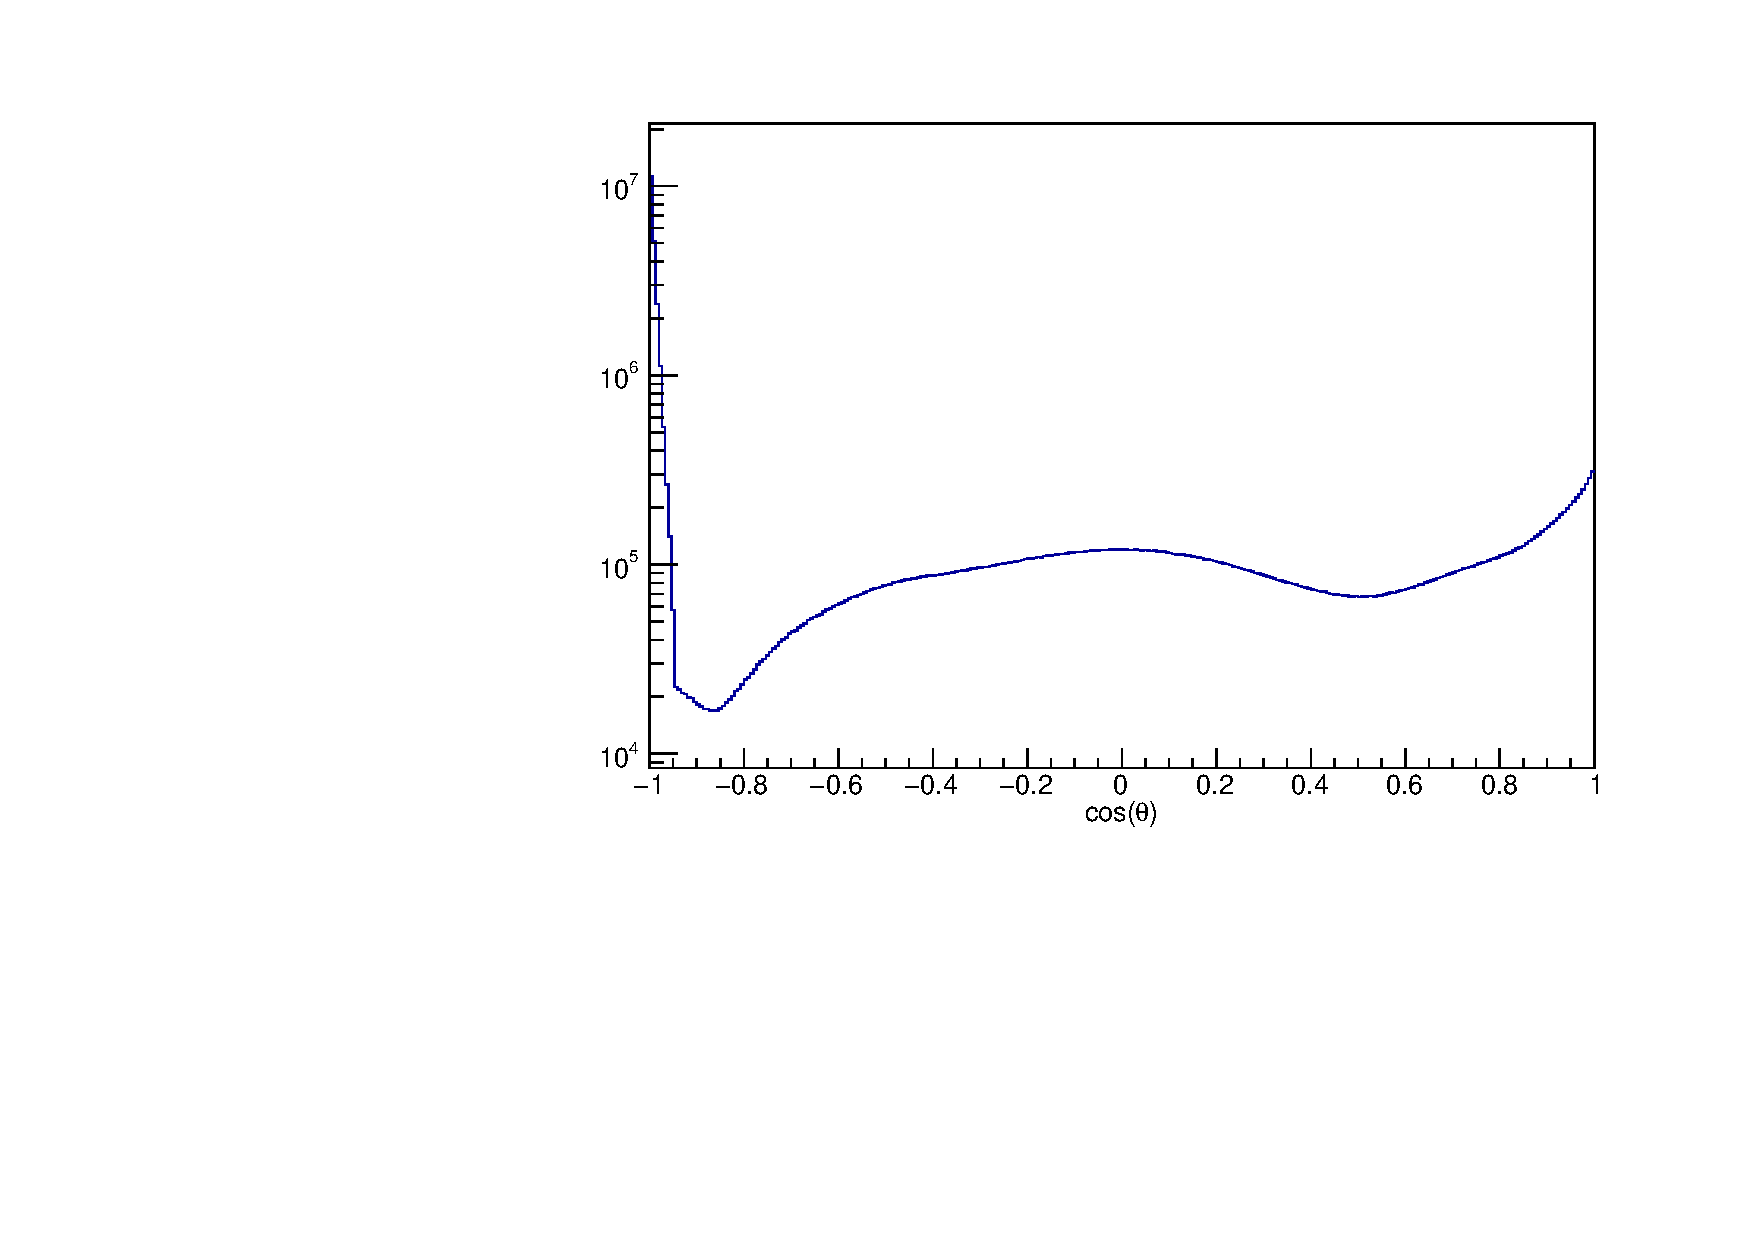
\includegraphics[width=\linewidth]{../figures/cosang.pdf}
	\caption{A histogram of all the mutual angles between all particles.}
	\label{fig:cosAll}
\end{figure}

By looking at this, we see that most of the angles will lie close to $180\degree$, and now we must decide exactly where to do the cutoff. 
By taking a sharp cutoff at $\cos(\theta) \geq -0.99$, we will exclude a great deal of good measurements, on the other hand, a too soft cut will not accomplish anything, as too many "wrong" particles will let through the check. 



\section{Momentum cut}
The second cut we perform on the data is a \textit{total} momentum cut. We see on \cref{fig:totalMomentum} the total momentum for the two identified \al-particles. 
A prominent peak lies around \note{SOME VALUE}, and ends around 40.000 keV. \note{SPØRG HANS OM HVORFOR 40k er godt, og hvad unit er}. Since there is still a large tail of higher momentum, we cut those out, and only get the particles we are sure can actually be \al-particles. 

\section{Multiplicity cut}
The last cut that we want to impose on the data, is a multiplicity cut. This cut is just to ensure that we have the amount of particles that we expect. 
Therefore a hard criteria is that there must be at least two distinctly identified \al-particles. \\

With regards to the \be-particles, we are more loose. Here we say that there must at least be one, but more can occur. This is quite rare, but the we still take that event into account, as the \be-particles should have an isotropic distribution, and therefore should not in any case be affected by the other \al-particles. On \cref{fig:betaMul} we see the multiplicity of \be-particles, and it is quite rare that there are more than one in a given event, so most of the time, we are in the expected case with two \al-particle and one \be-particle. 


\section{The properties of the \al-particles}


\section{Angular efficiency of the setup}
Since the detectors are unable to cover the entire solid angle, there will always be some mutual angles that are more likely to be measured. 
If we only look at one detector, a very large number of angles are not covered, but small mutual angles such as $\theta \approx 180\degree$, are very easy to measure, as it is just a measurement of two particles in the same pixel. 
This effect becomes apparant on \cref{fig:oneDetEff}, where the angular efficiency is shown for Det??. \\
In this setup however, we a cube of square detectors, who's normal vectors are all pointing in towards target at the center. This gives a much larger coverege of all mutual angles. 
The placement of the detectors gives that angles around $\theta \approx 90 \degree$ are also very favored. This makes sense, almost no matter what pixel was hit, there is a corresponding pixel $90\degree$ to both sides. On the same way, will there always be a corresponding pixel $\approx 180\degree$ from each pixels. This effect can be seen on \cref{fig:effAllDet}. \\
This histogram was created by using the spacial coordinates of the entire setup. First the positions of each pixel in each detector was found. Then two loops running over each pixel pair $i, j$, finds the angle between these pixels and saves it.\\


There is still a geometric effect that is not accounted for in the above analysis. We still need to consider that not all pixels in the detector has the same effective area. 
A pixel furthest out in a detector will have a effective area smaller than the area of a pixel in the center. This effect can be seen on \cref{fig:MexiHatDetector}. Here we see that \note{blalalala}\\
\\
To account for this effect, each pixel will be associated with a corresponding area-efficiency $(\text{Eff}_A)$.
This is calculated as 
\begin{equation}
\text{Eff}_A = \dfrac{\cos(\theta)}{r^2 },
\end{equation}
where $r$ is the distance to the pixel and $\theta$ is the angle between the inverted normal vector of the pixel and the line from the center to the pixel. A illustration of the scenario can be seen on \cref{fig:EffGeometry}.

On \cref{fig:effwithweight} two?? histograms can be seen. The red line represents the angular efficiency of the setup, without accounting for the relative area of the pixels, while the blue line is a weighted histogram for the same angles, with each pixels relative area accounted for. \\
The form of the two histograms are quite \note{bla bal bal} 
\begin{figure}[h]
	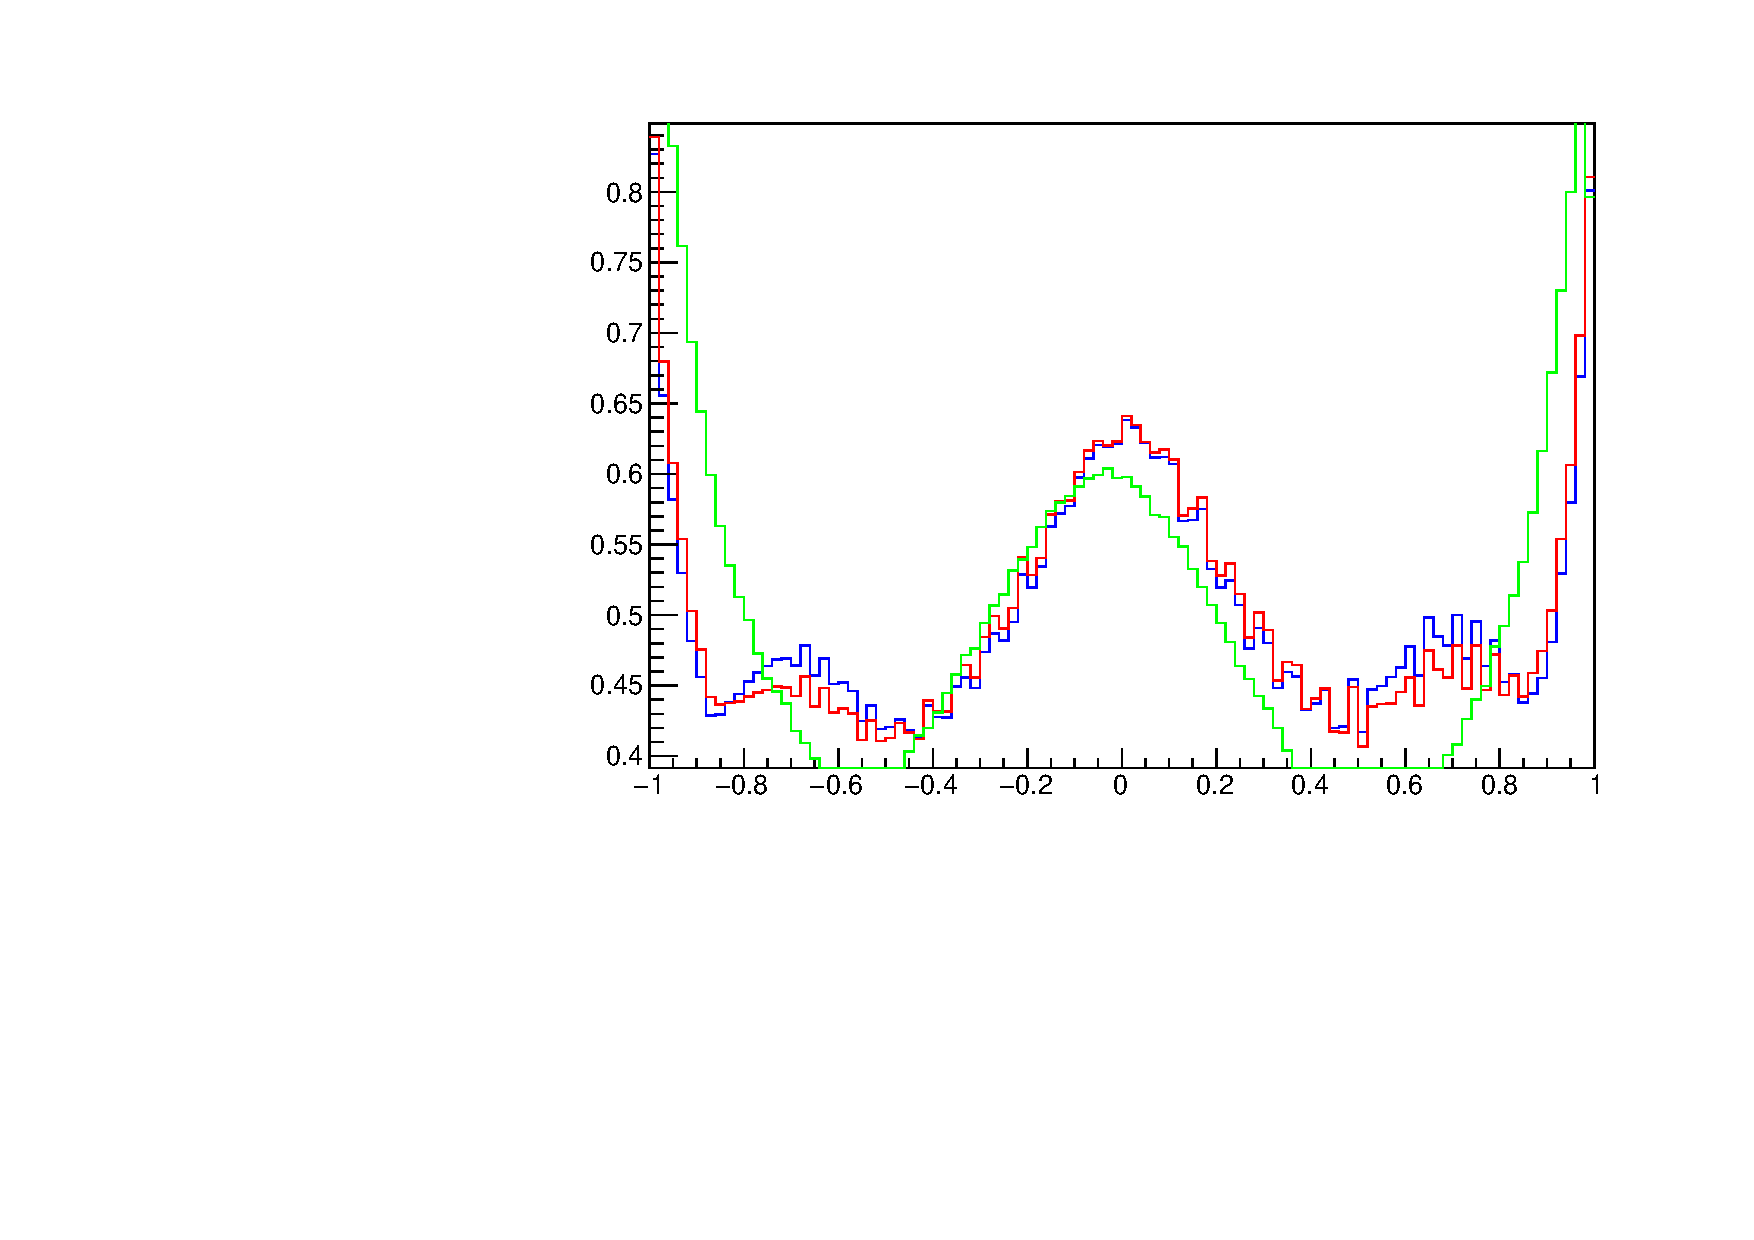
\includegraphics[width=\linewidth]{../figures/betaAngles/dataEffNormWithWeights.pdf}
	\caption{Some figure of the efficiency of the setup without efficiency of each pixel. }
	\label{fig:effwithweight}
\end{figure}


\section{Angular correlations of \al-particles and \be-particles}
From what we know in \note{ref til beta = isotrop} the \be-particles must have an isotropic distribution from the \al-particles. 

